\section{Nuclear recoil on the Born--Oppenheimer surface}\label{sec:19.1}

A silicon nucleus kicked with \SI{12.5}{eV} along $\langle111\rangle$ either swings out and returns to its site, or pushes a neighbor into the open tetrahedral site and leaves a defect behind (\cref{sec:7.4}). The nuclear response of \cref{chap:11} does not distinguish the two outcomes. It gives the rate of the kick and the energy $\omega$ deposited, and both are fixed before the struck atom has moved (\cref{sec:11.4}). Which outcome occurs is decided afterward, in some \SI{25}{fs}, by the motion of the struck atom between its neighbors on the Born--Oppenheimer surface $E^{\mathrm{ad}}$ of \cref{sec:5.1}. To follow this motion we need the state in which the response leaves the crystal, the regimes in which that state can be propagated by classical dynamics, and a definition of the shares into which the energy finally splits.

\subsection{The hand-over from the nuclear response}\label{sec:19.1-handover}

The kick either leaves the electrons in their ground state or also excites them. On the plane of the joint response of \cref{sec:12.1}, the line $\omega_e = 0$ holds the kicks after which the electrons stay in their ground state. It has the weight $1 - P_{\mathrm{Mig}}(q)$ of \cref{eq:12.1-zeroth} and the dressed mass $M_\kappa + \delta M_\kappa$; the remaining kicks form the Migdal entry, in which the same kick also leaves an electronic energy $\omega_e > 0$ (\cref{sec:12.1-counting}). Kicks on the line $\omega_e = 0$ and Migdal events set the nucleus moving with the same lattice factor. We follow the nucleus here, and a Migdal event hands its electronic energy to the cascade of \cref{chap:18} in addition. In silicon the weight $1 - P_{\mathrm{Mig}}$ differs from one by less than $10^{-3}$ for $E_R \lesssim \SI{16}{eV}$ and by \SI{1.9}{\percent} at \SI{500}{eV} with the exact second-order bracket, \SI{3}{\percent} in the soft limit (\cref{sec:12.1-counting,sec:12.3-validity}).

At small recoil parameter $x_R = E_R/\langle\omega\rangle$ the final states of the line $\omega_e = 0$ are states of a few phonons, and the response already resolves them by branch and momentum (\cref{eq:11.3-Sn}). Their energy $\omega$ goes as heat straight to the phonon readout (\cref{sec:8.7}). At $T > 0$ some terms of the response absorb a thermal phonon instead of creating one; they carry negative heat, and the net lattice energy, created minus absorbed, is $\omega$.

At large $x_R$ the response no longer lists phonons. In the impulse regime it is a peak of width $\sigma_\omega$ around the free recoil energy $E_R = q^2/2M_\kappa$ (\cref{eq:11.4-IA}), and the nucleus that received the kick moves far enough to collide with its neighbors. The state of the lattice after the kick is known exactly. Within the Born--Oppenheimer approximation the kick acts on the nuclear wave function alone, and multiplies it by $\ee^{\ii\vect{q}\cdot\vect{X}_I}$, with $\vect{X}_I$ the position of the struck nucleus $I$ of species $\kappa$. Write $\{\vect{X}\}$ and $\{\vect{p}\}$ for the positions and momenta of all nuclei, and describe the initial state $\varrho_0$ of the lattice, ground or thermal, by its Wigner function
\begin{equation*}
  \mathcal{W}_0(\{\vect{X}\},\{\vect{p}\}) = \int\frac{\dd\{\vect{y}\}}{(2\pi)^{3N}}\;\langle\{\vect{X} - \vect{y}/2\}|\varrho_0|\{\vect{X} + \vect{y}/2\}\rangle\,\ee^{\ii\sum_J\vect{p}_J\cdot\vect{y}_J} ,
\end{equation*}
whose marginals are the distributions of the positions and of the momenta. After the kick the density matrix is $\ee^{\ii\vect{q}\cdot\vect{X}_I}\varrho_0\,\ee^{-\ii\vect{q}\cdot\vect{X}_I}$. Its matrix element between $\{\vect{X} - \vect{y}/2\}$ and $\{\vect{X} + \vect{y}/2\}$ is that of $\varrho_0$ times $\ee^{\ii\vect{q}\cdot(\vect{X}_I - \vect{y}_I/2)}\ee^{-\ii\vect{q}\cdot(\vect{X}_I + \vect{y}_I/2)} = \ee^{-\ii\vect{q}\cdot\vect{y}_I}$. The extra phase shifts the momentum variable of the Fourier integral:
\begin{equation}
  \mathcal{W}_+(\{\vect{X}\},\{\vect{p}\}) = \mathcal{W}_0(\{\vect{X}\},\{\vect{p}\})\big|_{\vect{p}_I \to \vect{p}_I - \vect{q}} .
  \label{eq:19.1-wigner}
\end{equation}
The kick leaves every position where it was and moves the momentum of one nucleus by $\vect{q}$, for any $q$ and any potential.

The Hamiltonian of the nuclei is $H = \sum_J\vect{p}_J^2/2M_J + E^{\mathrm{ad}}(\{\vect{X}\})$, a function of the momenta plus a function of the positions. For a Hamiltonian of this form, the phase-space function that represents $H$ in the Wigner picture is the classical $H_{\mathrm{cl}}(\{\vect{X}\},\{\vect{p}\})$ itself. Every point of phase space therefore gains
\begin{equation}
  H_{\mathrm{cl}}(\{\vect{X}\},\{\vect{p}\} + \vect{q}\hat{\vect{e}}_I) - H_{\mathrm{cl}}(\{\vect{X}\},\{\vect{p}\}) = E_R + \frac{\vect{q}\cdot\vect{p}_I}{M_\kappa} ,
  \label{eq:19.1-dH}
\end{equation}
with $\hat{\vect{e}}_I$ marking the momentum of nucleus $I$. This is the energy $D$ that the kick gives a free particle of momentum $\vect{p}_I$ (\cref{sec:11.4}). Now let each point of $\mathcal{W}_+$ move along its classical trajectory on $E^{\mathrm{ad}}$. Since classical motion conserves $H_{\mathrm{cl}}$, each trajectory carries its deposited energy \cref{eq:19.1-dH} unchanged, and the distribution of the deposit over the ensemble is the distribution of $E_R + \vect{q}\cdot\vect{p}_I/M_\kappa$ over the momentum marginal $\mathfrak{f}_\kappa(\vect{p}_I)$. This distribution is the impulse approximation \cref{eq:11.4-IA}, term by term.
\begin{keyresult}[Recoil hand-over]
In the impulse regime, the nuclear response hands over the ensemble $\mathcal{W}_+$ of \cref{eq:19.1-wigner}: positions and momenta drawn from the Wigner function of the lattice before the kick, ground or thermal, with the momentum of the struck nucleus raised by $\vect{q}$. Propagated classically on $E^{\mathrm{ad}}$, the ensemble deposits $\omega = E_R + \vect{q}\cdot\vect{p}_I/M_\kappa$ per trajectory, and the distribution of this deposit reproduces \cref{eq:11.4-IA} with its exact mean $E_R$ and its exact width $\sigma_\omega$ of \cref{eq:11.4-width}. The hand-over misses the third cumulant $c_3$ of \cref{eq:D.32-c3}, which carries the force of the neighbors during the kick, and the quantum corrections to the motion after the kick.
\end{keyresult}
\noindent The two omissions set the validity of the hand-over. The share of $c_3$ in the shape of the peak falls as $x_R^{-1/2}$ (\cref{sec:11.4}). The quantum corrections to the trajectories are small once the recoil holds many vibrational quanta. \Cref{sec:19.1-regimes} makes this condition quantitative, and in silicon it holds above about \SI{0.4}{eV}. For a harmonic lattice the Wigner function is a positive Gaussian, at the zero-point widths at $T = 0$ and with the $\coth(\omega/2T)$ widths of \cref{sec:11.4} at $T > 0$, and it can be sampled point by point. Anharmonic zero-point distributions come from path-integral sampling (\cref{app:E.17}).

The struck atom starts with a spread of kinetic energies. At $T = 0$ the spread is $\sigma_\omega = (E_R\langle\omega\rangle)^{1/2}$. For silicon at the lowest displacement threshold, $E_R = \SI{12.5}{eV}$ with $\langle\omega\rangle = \SI{40.9}{meV}$, $\sigma_\omega$ is \SI{0.72}{eV}, or \SI{5.7}{\percent} of the threshold. A simulation that starts the other atoms at rest, as for a classical crystal at millikelvin, has no spread of kinetic energies. The direction of the recoil is that of $\vect{q}$ only on average. Let $E^{\mathrm{kin}}_\kappa = \langle\omega\rangle/4 = \SI{10.2}{meV}$ be the mean zero-point kinetic energy of the nucleus per Cartesian component (\cref{sec:11.4}). The transverse momentum of the struck nucleus then has the rms value $(2M_\kappa E^{\mathrm{kin}}_\kappa)^{1/2}$ per component, against the kick $q = (2M_\kappa E_R)^{1/2}$, so the recoil direction scatters by the rms angle $(E^{\mathrm{kin}}_\kappa/E_R)^{1/2}$ in each transverse plane: \SI{1.6}{\degree} at \SI{12.5}{eV}, or \SI{2.3}{\degree} in polar angle. And the displacement threshold becomes a smooth step. Let $\hat{\vect{r}}_R = \hat{\vect{q}}$ be the recoil direction and run every trajectory of the ensemble until its motion has been carried off into the lattice. The basin of the perfect crystal on $E^{\mathrm{ad}}$ is the set of configurations that relax to it. The probability $p_{\mathrm{FP}}(E_R, \hat{\vect{r}}_R)$ that the end state lies outside this basin, in a Frenkel pair (FP) or another defect, rises from 0 to near 1 over a range of $E_R$, and we take as the displacement threshold the lowest $E_R$ at which $p_{\mathrm{FP}}$ reaches one half,
\begin{equation}
  E_{\mathrm{d}}(\hat{\vect{r}}_R) = \min\bigl\{E_R :\ p_{\mathrm{FP}}(E_R, \hat{\vect{r}}_R) \ge \tfrac12\bigr\} .
  \label{eq:19.1-Ed}
\end{equation}
When every trajectory of the ensemble is the same, $p_{\mathrm{FP}}$ is a step function and \cref{eq:19.1-Ed} is the deterministic threshold \cref{eq:7.4-Ed}. The spread $\sigma_\omega$ of the deposit spreads the step over about \SI{0.7}{eV} in silicon, before the spread of the initial positions adds its own; the measured onset of damage, $12.9 \pm \SI{0.6}{eV}$~\cite{loferski1958radiation}, carries an uncertainty of the same size. The step width is a prediction of the response and not a parameter of the dynamics. It matters for light dark matter, whose recoil spectrum falls steeply near its endpoint, so that the few recoils above $E_{\mathrm{d}}$ lie on the edge of the step.

\subsection{Regimes of the recoil dynamics}\label{sec:19.1-regimes}

Whether the handed-over ensemble may be propagated classically, harmonically, without defects and without electronic excitation is decided by four numbers: the quantum ratio $\lambda_{\mathrm{dB}}/\ell_R$, the anharmonic ratio $\eta_R$, the displacement threshold $E_{\mathrm{d}}$ and the Massey parameter $\xi_{\mathrm{M}}$. Each compares a property of the struck atom at kinetic energy $E_R$ with a scale of the crystal, and \cref{fig:19-recoil}(b) plots them for silicon.

The quantum and the anharmonic numbers use the amplitude of the struck atom's first excursion. Before its energy has spread, the atom moves in the cage of neighbors that have not yet responded, and for an estimate we treat that cage as an oscillator of the mean phonon frequency. The turning point of the struck atom lies at
\begin{equation*}
  \ell_R = \Bigl(\frac{2E_R}{M_\kappa\langle\omega\rangle^2}\Bigr)^{1/2} ,
\end{equation*}
from $E_R = \tfrac12M_\kappa\langle\omega\rangle^2\ell_R^2$. Classical mechanics holds when the de Broglie wavelength $\lambda_{\mathrm{dB}} = 2\pi/(2M_\kappa E_R)^{1/2}$ is short compared with this amplitude. The ratio is
\begin{equation*}
  \frac{\lambda_{\mathrm{dB}}}{\ell_R} = \frac{2\pi}{(2M_\kappa E_R)^{1/2}}\Bigl(\frac{M_\kappa\langle\omega\rangle^2}{2E_R}\Bigr)^{1/2} = \frac{\pi\langle\omega\rangle}{E_R} ,
\end{equation*}
independent of the mass: the motion is classical when the recoil holds many quanta $\langle\omega\rangle$. The corrections to classical trajectories are of second order in $\hbar$, and we take their relative size to be $(\lambda_{\mathrm{dB}}/\ell_R)^2$, an estimate. The harmonic approximation holds when $\ell_R$ is short compared with the length $3\Phi^{(2)}/|\Phi^{(3)}|$ over which the force constants change by their own size. The ratio of $\ell_R$ to this length is the anharmonic parameter $\eta_{\mathrm{anh}}$ of \cref{eq:5.7-eta} with the recoil amplitude in place of the zero-point length,
\begin{equation*}
  \eta_R = \frac{|\Phi^{(3)}|\,\ell_R}{3\Phi^{(2)}} ,
\end{equation*}
and by the counting of \cref{eq:5.7-order} the anharmonic corrections to energies and widths are of order $\eta_R^2$. For silicon, the bond-coordinate values of \cref{sec:5.7} give $3\Phi^{(2)}/|\Phi^{(3)}| = \SI{0.98}{\angstrom}$.

The third number is the displacement threshold itself: below $E_{\mathrm{d}}(\hat{\vect{r}}_R)$ the trajectory relaxes back into the basin of the perfect crystal, above it a defect survives with probability $p_{\mathrm{FP}}$. The fourth number decides whether the electrons follow. A nucleus at speed $v_N = (2E_R/M_\kappa)^{1/2}$ changes the potential seen by the electrons over a time $\ell_{\mathrm{int}}/v_N$, with $\ell_{\mathrm{int}} \approx \SI{1}{\angstrom}$ the range over which a close collision distorts the bonds. The electrons follow adiabatically if this time is long compared with $1/\Eg$, the time scale of the lowest excitation. The ratio of the two times is the Massey parameter
\begin{equation*}
  \xi_{\mathrm{M}} = \frac{\Eg\,\ell_{\mathrm{int}}}{v_N} ,
\end{equation*}
and for a perturbation that is smooth on the scale $\ell_{\mathrm{int}}$ the probability of an electronic transition falls as $\ee^{-\xi_{\mathrm{M}}}$. The bulk gap overstates the adiabaticity of a close collision, since the local gap of the compressed pair closes as the atoms approach, and \cref{sec:19.2} treats electronic excitation in close collisions.

\begin{figure}[tbp]
  \centering
  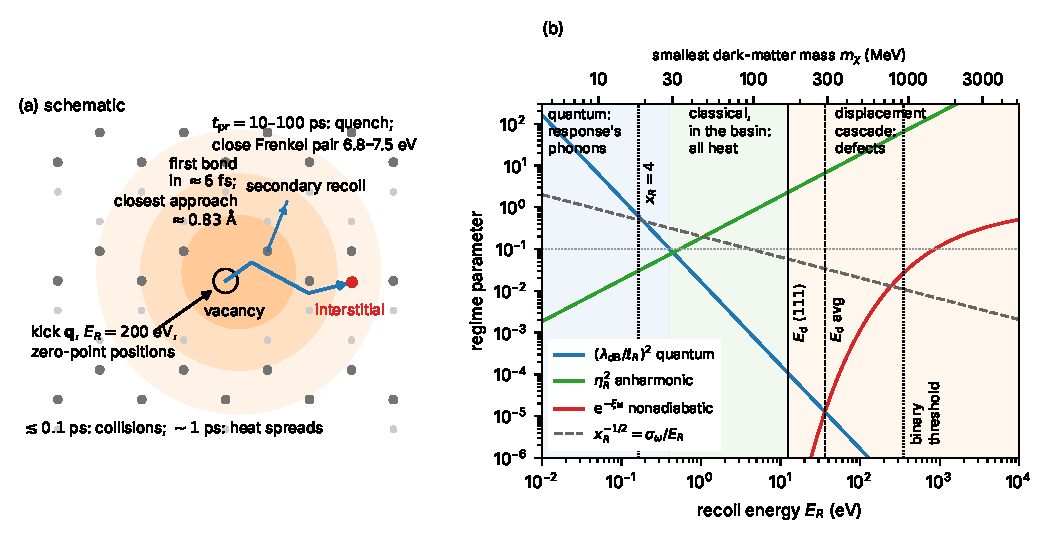
\includegraphics[width=\linewidth]{figures/ch19/fig19_1.pdf}
  \caption{A silicon nuclear recoil after the hand-over. (a) Schematic of a \SI{200}{eV} recoil in a $(1\bar10)$ plane of the diamond lattice (dark dots: atoms in the plane; light dots: the neighboring planes). The kick starts the struck atom from its zero-point position; it crosses its first bond in about \SI{6}{fs}, with a closest approach of \SI{0.83}{\angstrom} in a head-on collision, and sets a secondary atom moving. Within about \SI{0.1}{ps} the collisions are over, and within about a picosecond the heat (shaded rings) spreads through the crystal. At the partition time $t_{\mathrm{pr}}$ of \cref{sec:19.1-partition}, 10 to \SI{100}{ps}, the end state is quenched: here a vacancy and an interstitial, which as a close Frenkel pair store 6.8 to \SI{7.5}{eV}. Paths and end positions are drawn by hand. (b) The regime parameters against the recoil energy $E_R$ at $T = 0$. Curves: the quantum correction $(\lambda_{\mathrm{dB}}/\ell_R)^2 = (\pi\langle\omega\rangle/E_R)^2$, the anharmonic parameter $\eta_R^2$ with $3\Phi^{(2)}/|\Phi^{(3)}| = \SI{0.98}{\angstrom}$, the adiabatic suppression $\ee^{-\xi_{\mathrm{M}}}$ with $\Eg = \SI{1.17}{eV}$ and $\ell_{\mathrm{int}} = \SI{1}{\angstrom}$, and the relative width $x_R^{-1/2} = \sigma_\omega/E_R$ of the handed-over deposit, with $\langle\omega\rangle = \SI{40.9}{meV}$. The dotted horizontal line is the criterion 0.1. Vertical lines: impulse onset $x_R = 4$, displacement thresholds \SI{12.5}{eV} ($\langle111\rangle$) and \SI{36}{eV} (Frenkel pair, direction average), and the binary electron--hole threshold \SI{352}{eV} of \cref{sec:19.2}. Shading: quantum regime, where the phonons of the response are the final state (blue); classical motion inside the basin of the perfect crystal, where all energy becomes heat (green); displacement cascade (orange). Top axis: the smallest dark-matter mass that reaches $E_R$ at $v_{\mathrm{max}} = 2.650\times10^{-3}$.}
  \label{fig:19-recoil}
\end{figure}

The numbers divide the recoil energies into a quantum, a classical, a displacement and a nonadiabatic regime. The boundaries between the regimes follow from the definitions of the four numbers. Their positions depend on the criterion and on the cage estimate, and we quote them as estimates for a criterion of 0.1.
\begin{description}
\item[Quantum.] For $(\pi\langle\omega\rangle/E_R)^2 > 0.1$, that is $E_R < \pi\langle\omega\rangle/\sqrt{0.1}$, the recoil holds too few quanta for classical motion. The response is the whole answer here: its phonons are the final state and the energy is heat.
\item[Classical, inside the basin.] From the upper edge of the quantum regime up to $E_{\mathrm{d}}$ the motion is classical and adiabatic, anharmonic above $\eta_R^2 = 0.1$, and the trajectory relaxes back to the perfect crystal. Born--Oppenheimer molecular dynamics is controlled, and all of the energy becomes heat. The dynamics adds to the response the spectrum of the phonons the recoil leaves, which anharmonic collisions redistribute.
\item[Displacement cascade.] Above $E_{\mathrm{d}}$ some trajectories end in a defect, and the energy splits into heat and stored energy. A recoil many times $E_{\mathrm{d}}$ sets secondary atoms moving above their own thresholds and so starts the collision cascade of \cref{fig:19-recoil}(a).
\item[Nonadiabatic.] Where $\ee^{-\xi_{\mathrm{M}}}$ is no longer negligible, the electrons are excited along the path, and part of the energy becomes charge.
\end{description}
The quantum and harmonic boundaries lie close together: in silicon there is no wide window in which the motion is both harmonic and classical. The hand-over, however, does not need the motion to be harmonic. It takes place at the instant of the kick, and its only requirement on the later motion is that the motion be classical.

\begin{workedexample}{Regime boundaries for silicon}\label{we:19-boundary}
A silicon nucleus of the natural isotope mixture has $M_\kappa = 28.0855\,\mathrm{u} = \SI{26.16}{GeV}$, as in \cref{sec:5.3}, and $\langle\omega\rangle = \SI{40.9}{meV}$ (\cref{sec:11.4}). The cage stiffness is $M_\kappa\langle\omega\rangle^2 = \SI{26.16}{GeV}\times(\SI{0.0409}{eV})^2/(\hbar c)^2 = \SI{11.24}{eV.\angstrom^{-2}}$, with $\hbar c = \SI{1973.27}{eV.\angstrom}$.

\emph{Classical boundary.} $(\pi\langle\omega\rangle/E_R)^2 = 0.1$ gives $E_R = \pi\times\SI{0.0409}{eV}/0.316 = \SI{0.41}{eV}$, or $x_R = 9.9$. At \SI{1}{eV}, $\lambda_{\mathrm{dB}} = \SI{0.054}{\angstrom}$ against $\ell_R = \SI{0.42}{\angstrom}$, and the correction estimate is 0.017.

\emph{Harmonic boundary.} $\eta_R^2 = 0.1$ means $\ell_R = 0.316\times\SI{0.98}{\angstrom} = \SI{0.31}{\angstrom}$, reached at $E_R = \tfrac12\times\SI{11.24}{eV.\angstrom^{-2}}\times(\SI{0.31}{\angstrom})^2 = \SI{0.54}{eV}$. At \SI{1}{eV}, $\eta_R^2 = 0.18$.

\emph{Displacement.} The lowest threshold is \SI{12.5}{eV} along $\langle111\rangle$, the direction average for a Frenkel pair \SI{36}{eV}~\cite[Table~IV]{holmstrom2008threshold}. At \SI{12.5}{eV} the cage amplitude is $\ell_R = \SI{1.49}{\angstrom}$, more than half the bond length of \SI{2.35}{\angstrom}: the cage estimate has run out, as it should, since the atom is leaving its cage. The atom moves at $v_N = \SI{9.27}{km/s}$ and crosses one bond in \SI{25}{fs}, less than half the shortest phonon period of \SI{65}{fs} ($2\pi/\omega_{\mathrm{opt}}$ with $\omega_{\mathrm{opt}} = \SI{64.1}{meV}$, \cref{sec:5.7}), so the collision is over before the lattice has responded. The energy ends in some $\SI{12.5}{eV}/\langle\omega\rangle \approx 300$ phonons if no defect survives.

\emph{Adiabaticity.} At \SI{20}{eV}, $v_N = \SI{11.7}{km/s}$ and $\xi_{\mathrm{M}} = \SI{1.17}{eV}\times\SI{1}{\angstrom}/(\hbar v_N) = 15$, with $\hbar = \SI{6.582e-16}{eV.s}$, so $\ee^{-\xi_{\mathrm{M}}} = 3\times10^{-7}$. Since $\xi_{\mathrm{M}} \propto E_R^{-1/2}$, the suppression reaches 0.1 ($\xi_{\mathrm{M}} = 2.3$) at \SI{0.87}{keV}, and $\xi_{\mathrm{M}} = 1$ at \SI{4.6}{keV}.

\emph{Dark-matter masses.} By \cref{eq:1.3-ERmax} with $v_{\mathrm{max}} = 2.650\times10^{-3}$, the classical boundary needs $\mchi \ge \SI{28}{MeV}$, the harmonic boundary \SI{32}{MeV}, the lowest threshold \SI{154}{MeV}, the average threshold \SI{262}{MeV}, and $\ee^{-\xi_{\mathrm{M}}} = 0.1$ needs \SI{1.3}{GeV}.
\end{workedexample}


\subsection{Acceptance tests for recoil molecular dynamics}\label{sec:19.1-md}

In the classical regimes the handed-over ensemble is propagated by molecular dynamics on $E^{\mathrm{ad}}$. A recoil cascade needs cells of thousands of atoms and thousands of trajectories, far beyond direct density-functional dynamics. In practice the surface is therefore a machine-learned interatomic potential, trained on density-functional energies and forces and joined to a screened Coulomb repulsion at short distance. \Cref{app:E.11} describes the method.

The energy surface must be right along the path of the struck atom, not only near equilibrium. The threshold is set by the energy surface between the neighbors that the struck atom squeezes past. Potentials that agree on elastic constants and defect energies can still disagree on thresholds by several eV; the Stillinger--Weber potential overshoots the density-functional threshold along $\langle111\rangle$ by 4 to \SI{6}{eV} (\cref{sec:7.4}). The accuracy target is the width of the step in $p_{\mathrm{FP}}$, about \SI{0.7}{eV} at the lowest silicon threshold, checked against density-functional dynamics along a few directions. Closer in, the closest approach of a head-on collision is \SI{1.49}{\angstrom} at \SI{20}{eV} and \SI{0.83}{\angstrom} at \SI{200}{eV} (\cref{tab:E-md-si}). At these distances the screened Coulomb repulsion dominates, and the splice between the machine-learned potential and the screened Coulomb repulsion must be complete above the turning point of threshold collisions, so that the dynamics near $E_{\mathrm{d}}$ never feels the splice.

The initial ensemble must be the kicked zero-point ensemble of the hand-over, not a lattice at rest. Classical propagation of a Wigner ensemble is exact for a quadratic Hamiltonian, since the quantum evolution of the Wigner function then reduces to the classical Liouville flow. The zero-point motion of the parts of the crystal that stay harmonic is therefore carried correctly. Where the collision makes the surface anharmonic, classical dynamics lets the zero-point energy of one mode flow into others and leaves the mode below its quantum ground state, a state that quantum dynamics forbids. The error from this leakage is of the order of the zero-point energy of the atoms the collision disturbs, a few tens of meV each, and the definition of the stored energy below is built so that the error does not enter.

The stored energy must be measured between minima. On average, each atom of the initial ensemble lies above the minimum of $E^{\mathrm{ad}}$ by half its zero-point energy, $3\langle\omega\rangle/4 = \SI{31}{meV}$ per atom in silicon (the zero-point energy of \cref{sec:5.3} is \SI{123}{meV} per cell of two atoms). In a cell of 4096 atoms this excess is \SI{126}{eV}, more than ten times the energy of a Frenkel pair. The end state and the perfect crystal are therefore both relaxed to their minima, by a quench at fixed cell without annealing, and the stored energy is the difference \cref{eq:E.11-Est}. The potential's own error on defect energies sets a floor: a potential whose formation energies lie within \SI{7}{\percent} of density-functional theory~\cite[Sect.~III\,E]{bartok2018machine} carries an error of a few tenths of an eV on a defect that stores several eV. One table of these minimum energies, with one potential and cell, must serve the stored energy of \cref{sec:19.4} and the release paths of \cref{sec:19.6}, or the two disagree by that error.

The harmonic limit provides an acceptance test. With $E^{\mathrm{ad}}$ replaced by its harmonic expansion, the classical propagation of $\mathcal{W}_+$ is exact. The mean energy that the kick leaves in a normal mode $s$ is then $|\vect{q}\cdot\vect{e}_{\kappa s}|^2/2NM_\kappa$, with $\vect{e}_{\kappa s}$ the polarization vector of the mode on the struck site and $N$ the number of cells. It is half the square of the mass-weighted momentum the kick gives the mode, since the cross term with the mode's own momentum averages to zero over the ensemble. These mode energies sum to $E_R$ by the completeness of the polarization vectors, and they are the energy-weighted phonon content of the harmonic response of \cref{sec:11.3} at the same $\vect{q}$. A calculation that propagates the kicked ensemble on the true surface must recover this spectrum for recoils small enough to stay harmonic, and the mean and width of \cref{eq:11.4-IA} for all others.

The electronic channel is missing from Born--Oppenheimer dynamics. A common remedy adds a friction force, minus the electronic stopping power times the direction of motion. Below the binary threshold of \cref{sec:19.2} that friction fails (\cref{sec:19.3-assumptions}), and at any energy it supplies a mean loss without its distribution. Where the electronic channel matters, the friction is replaced by excitation events drawn at each close collision from a kernel computed with time-dependent density-functional theory (\cref{sec:19.2}).

\subsection{Partition of the recoil energy}\label{sec:19.1-partition}

The shares of the recoil energy change with time, and the partition needs a time. The collisions are over within about \SI{0.1}{ps}, and the hot carriers that the recoil excites finish their cascade within a picosecond (\cref{chap:18}). Defects at millikelvin, on the other hand, cannot cross barriers of chemical size by thermal activation, since a barrier of \SI{0.1}{eV} at \SI{10}{mK} carries the Boltzmann factor $\ee^{-1.2\times10^5}$ (\cref{sec:7.4}); they move only by tunneling or with the phonons of later events (\cref{sec:19.6}). The drift of the pairs to the electrodes takes longer still (\cref{sec:20.1}). Any time $t_{\mathrm{pr}}$ between 10 and \SI{100}{ps} after the recoil comes after the collisions and the hot-carrier cascade and before any defect motion or pair drift, and we fix the partition there.

At $t_{\mathrm{pr}}$ the energy $\omega$ deposited in the kick has gone three ways. Part has gone to the electrons: the energy $\omega_e$ of a Migdal event, if the kick was one, plus whatever the moving nucleus excited along its path. The nuclei keep the rest of $\omega$, as kinetic energy and as potential energy on $E^{\mathrm{ad}}$. The quench at $t_{\mathrm{pr}}$ splits the nuclear share into the energy of the minimum that the crystal has reached and the vibrational energy about that minimum.
\begin{keyresult}[Partition of the recoil energy]
At the time $t_{\mathrm{pr}}$,
\begin{equation}
  \omega = E_{\mathrm{lat}} + E_{\mathrm{st}} + \omega_e , \qquad
  E_{\mathrm{st}} = E^{\mathrm{ad}}_{\mathrm{min}}(\mathrm{end}) - E^{\mathrm{ad}}_{\mathrm{min}}(\mathrm{perfect}) ,
  \label{eq:19.1-partition}
\end{equation}
where $\omega_e$ is the energy given to the electrons and $E_{\mathrm{st}}$ the stored energy, the difference of the minima of $E^{\mathrm{ad}}$ in the basin of the end state and in that of the perfect crystal. The lattice share $E_{\mathrm{lat}}$ is the vibrational energy in excess of the zero-point energy of the perfect crystal. After the cascade of \cref{chap:18} has turned $\omega_e$ into $N_{\mathrm{eh}}$ pairs,
\begin{equation}
  \omega = N_{\mathrm{eh}}\Eg + E_{\mathrm{heat}} + E_{\mathrm{st}} , \qquad
  E_{\mathrm{heat}} = E_{\mathrm{lat}} + \bigl(\omega_e - N_{\mathrm{eh}}\Eg\bigr) .
  \label{eq:19.1-heat}
\end{equation}
\end{keyresult}
\noindent The energy balance follows from the conservation of the total energy along each trajectory. Before the kick the nuclei hold the minimum of the perfect crystal and its zero-point energy; the kick adds $\omega$, and the electrons take away $\omega_e$. At $t_{\mathrm{pr}}$ the nuclei hold the minimum of the end basin and the vibrational energy about it, and subtracting the balance before the kick from the balance at $t_{\mathrm{pr}}$ gives \cref{eq:19.1-partition}. The second form uses the cascade identity \cref{eq:18.1-energy} for each electronic excitation, $\omega_e = N_{\mathrm{eh}}\Eg + E_{\mathrm{heat}}$ of the cascade, and collects all phonon energy, from the lattice and from the cascade, in one $E_{\mathrm{heat}}$. For an electronic deposit, with $E_{\mathrm{lat}} = E_{\mathrm{st}} = 0$, the second form is \cref{eq:18.1-energy} itself. Capture at the end of the cascade moves energy out of the pairs as in \cref{sec:18.5}.

The stored energy is configurational: it compares minima of $E^{\mathrm{ad}}$ and contains no vibrational energy. The zero-point energy of the end basin differs from that of the perfect crystal, since a defect softens or stiffens the modes around it, and the difference is part of $E_{\mathrm{lat}}$, on the vibrational side. This zero-point difference is part of the heat but cannot reach a sensor, and \cref{sec:19.5} counts it separately. The stored energy is also not the displacement threshold, which is a barrier on the path rather than a difference of end points. A close Frenkel pair keeps about half of the lowest silicon threshold, and the rest of the threshold energy becomes heat (\cref{sec:7.4}).

The partition is random. Each trajectory of the handed-over ensemble ends with its own $(E_{\mathrm{lat}}, E_{\mathrm{st}}, \omega_e)$, and in the impulse regime the ensemble is fixed by $E_R$, the direction $\hat{\vect{r}}_R$ and the temperature. The cascade turns the electronic excitations into pairs with the distribution $P_{\mathrm{casc}}$ of \cref{sec:18.3}, evaluated at the seed energies the recoil produced, which lie near the gap. The result is a joint distribution $P(E_{\mathrm{heat}}, E_{\mathrm{st}}, N_{\mathrm{eh}}|E_R, \hat{\vect{r}}_R, T)$. Its correlations matter as much as its means, since a recoil that stores energy in a defect leaves less heat and, through the same collision, may give fewer pairs.

Below $E_{\mathrm{d}}$ the adiabatic suppression makes $\omega_e$ negligible, $\ee^{-\xi_{\mathrm{M}}} = 5\times10^{-9}$ at \SI{12.5}{eV}, and every trajectory returns to the perfect crystal, so the recoil deposits all of its energy as heat. In silicon the recoils below $E_{\mathrm{d}}$ include every electron-following recoil from dark matter below about \SI{150}{MeV} (\cref{we:19-boundary}). The charge that these recoils produce therefore comes from the Migdal entry of the response and from the soft tail of electronic excitation of \cref{sec:19.2}, not from the recoil dynamics. After $t_{\mathrm{pr}}$ the stored energy decreases as defects release it, and the pairs recombine or are collected; the balance law of \cref{sec:19.5} carries this time dependence, with \cref{eq:19.1-partition} as its starting point.
